\documentclass[a4paper, 12pt,oneside]{article} 
%\documentclass[a4paper, 12pt,oneside,draft]{article} 

\usepackage{preamble}
\usepackage{bm}
%--------------------- ACTUAL FILE ---------------------- %
\begin{document} 
%%%
	%\thispagestyle{empty}
	%\vspace*{\fill}
	\begin{center}
	    \Large
	    \textbf{Orthogonalization Techniques for a Set of Vectors}
	        
	    \vspace{0.4cm}
	    \large
		HPC for numerical methods and data analysis \\
	    Student : Tara Fjellman \\
	    \small{Fall 2024}
	\end{center}
	\section{Introduction}
	QR factorization is a fundamental operation in numerical linear algebra. It is used in many applications, such least squares problems, computing the low rank approximation of a matrix, and computing an orthogonal basis of a set of vectors. Its ``thin'' $Q$ version is defined as the factorization of a matrix ${A}\in \mathbb{R}^{m \times n}$ into the product of an orthogonal matrix ${Q}\in {R}^{m \times n}$ and an upper triangular matrix ${R}\in \mathbb{R}^{n \times n}$, such that ${A} = {Q} {R}$. The QR factorization can be computed using different algorithms, such as Classical Gram-Schmidt (CGS), Cholesky-QR, and Tall-Skinny QR (TSQR). These algorithms have different numerical properties and computational costs, which makes them suitable for different applications. In this project, we study the numerical stability and computational performance of these algorithms for orthogonalizing a set of vectors. We compare the algorithms using theoretical analysis and numerical experiments on two different matrices : a well conditioned one, and an ill-conditioned one. The goal is to identify an algorithm that is numerically stable and computationally efficient for orthogonalizing a set of vectors.

	In this project we consider $m \gg n$ and typically take $n$ between 50 and a few hundreds, while $m$ can be much larger.
	\section{Algorithms}
		\subsection{Classical Gram-Schmidt}
			Given a set of linearly independent vectors $A_1, \ldots, A_n \in \mathbb{R}^m$, the Gram-Schmidt algorithm computes an orthogonal basis $Q_1, \ldots, Q_n \in \mathbb{R}^m$ by orthogonalizing the vectors one by one. At the step $i$ of the algorithm, the $i$th vector $a_j$ is projected onto the orthogonal complement of the space spanned by the previous vectors $Q_1, \ldots, Q_{i-1}$, and the resulting vector is normalized to obtain $Q_i$.

			CGS is obtained by approximating the projector $I-Q(:,1:i)Q^\dagger(:,1:i)$ by $I-Q(:,1:i)Q^T(:,1:i)$. This corresponds to assuming $[Q(:,1:i)^TQ(:,1:i)]^{-1}=I$, i.e. that no numerical errors are committed during the orthogonalisation process. 
		\subsection{Cholesky-QR}
			The Cholesky-QR algorithm consists in computing $Q=AR^{-1}$ with $R$ found with help of the Cholesky decomposition of $A^TA$. The Cholesky decomposition of a matrix ${G}$ is a factorization of the form ${G} = {L} {L}^T$, where ${L}$ is a lower triangular matrix. Indeed, the Cholesky decomposition $A^TA=LL^T$ gives $R=L^T$ since $(QR)^T(QR)=R^TR\iff Q^TQ=I$. 
			
			Notice that in practice, instead of inverting $R$ we can solve for each column of $A^T$ the system associated to $R^TQ^T=A^T$ taking advantage of the triangular structure of $R$.
		\subsection{TSQR}
		%Remember that communication refers to messages between processors. In the recent years we've seen trends causing floating point to become faster than communication. This is why it's important to minimize communication when dealing with parallelism.
		The TSQR, ``Tall Skinny QR'' algorithm is a communication avoiding algorithm for matrices with many more rows than columns. 
		To better understand how it works, we first explain it assuming we were using P = 4 processors, therefore scattering row wise our matrix $A$ along 4 processors $A_1, A_2, A_3, A_4 \in \mathbb{R}^{m / 4 \times n}$. We will then explain how to generalise to the more general case. 
		
		The computation can be expressed as a product of intermediate orthonormal factors in a binary tree like structure.

		At the leaves of the binary tree, we perform in parallel 4 local QR factorizations to get $A_1=\hat{Q}_1^{(2)} \hat{R}_1^{(2)}, A_2=\hat{Q}_2^{(2)} \hat{R}_2^{(2)}, A_3=\hat{Q}_3^{(2)} \hat{R}_3^{(2)}, A_4=\hat{Q}_4^{(2)} \hat{R}_4^{(2)}$. Here $\hat{Q}_l^{(2)} \in \mathbb{R}^{m / 4 \times m / 4}$ and $\hat{R}_l^{(2)} \in \mathbb{R}^{m / 4 \times n}$. As we only are interested in the thin $Q$ factor for this application, we can work with the $Q_i^{(k)}\in\mathbb R^{m/4\times n}, R_i^{(k)}\in\mathbb R^{n\times n}$ instead of the full $\hat Q_i^{(k)}, \hat R_i^{k}$ ones. In block structure we therefore get
		$$
		\left[\begin{array}{l}
		A_0 \\
		A_1 \\
		A_2 \\
		A_3
		\end{array}\right]=\left[\begin{array}{llll}
		{Q}_0^{(2)} & & & \\
		& {Q}_1^{(2)} & & \\
		& & {Q}_2^{(2)} & \\
		& & & {Q}_3^{(2)}
		\end{array}\right]\left[\begin{array}{l}
		{R}_0^{(2)} \\
		{R}_1^{(2)} \\
		{R}_2^{(2)} \\
		{R}_3^{(2)}
		\end{array}\right]
		$$
		In the second level of the binary tree we combine the upper triangular matrices $R_0^{(2)}$ with $R_1^{(2)}$ and $R_2^{(2)}$ with $R_3^{(2)}$ to get block structured matrices. We perform the QR factorization in parallel to get $Q_{00}^{(1)},Q_{10}^{(1)},R_0^{(1)},Q_{22}^{(1)},Q_{32}^{(1)},R_2^{(1)}$ such that
		$$
		\left[\begin{array}{c}
		R_0^{(2)} \\
		R_1^{(2)}
		\end{array}\right]=\left[\begin{array}{c}
		{Q}_{00}^{(1)} \\
		{Q}_{10}^{(1)} 
		\end{array}\right]
		R_0^{(1)} 
		\quad\left[\begin{array}{c}
		R_2^{(2)} \\
		R_3^{(2)}
		\end{array}\right]=\left[\begin{array}{c}
		{Q}_{22}^{(1)} \\
		{Q}_{32}^{(1)}
		\end{array}\right]
		R_3^{(1)}.
		$$
		This can be written as
		$$
		\left[\begin{array}{c}
		{R}_0^{(2)} \\
		{R}_1^{(2)} \\
		{R}_2^{(2)} \\
		{R}_3^{(2)}
		\end{array}\right]=\left[\begin{array}{ccc}
			{Q}_{00}^{(1)} & & \\
			{Q}_{10}^{(1)} & & \\
			& & {Q}_{22}^{(1)} \\
			& & {Q}_{32}^{(1)} 
		\end{array}\right]\left[\begin{array}{c}
		R_0^{(1)} \\
		R_2^{(1)}
		\end{array}\right].
		$$
		Finally at the root of the tree we compute the last QR factorization
		$$
		\left[\begin{array}{c}
		R_0^{(1)} \\
		R_2^{(1)}
		\end{array}\right]=\left[\begin{array}{c}
			{Q}_{00}^{(0)} \\
			{Q}_{20}^{(0)}
		\end{array}\right]
		R_0^{(0)}
		$$
		After all this, one can write ${Q}=Q^{(2)}Q^{(1)}Q^{(0)}$.

		In the more general case, where $A$ is distributed over $2^P$ processors, we would have $P+1$ levels in the binary tree. The $Q^{(P)}$ matrix would still be block diagonal, but with $P$ blocks of size $m/P\times n$. The other $Q^{(q)}, q=P-1,...,0$ matrices would also be block diagonal, composed of $2^q$ blocks, each of size $2n\times n$. 
		The reduction tree used was obtained with the following procedure at every stage $q$ :
		(a) processors $i$ such that $i\mod 2^{P-q}=0$ are kept active; (b) processor $j$ for which $j\mod 2^{P-q+1}=1$ sends its data to processor $i=j-2^{P-q}$; (c) processor $i$ receives data from processor $j=i+2^{P-q}$. This method nicely generalises the reduction tree used in the 4 processor example. 

		Notice that TSQR's communication is minimal as no data is duplicated and the reduction tree is used to combine the results of the local QR factorizations.
	\section{Parallelisation}
		For parallelization of all the considered algorithms, the matrix ${A}$ is row-distributed over the processors. Each processor $i=0,...,P-1$ owns a block ${A}_i$.
		
		In the following sections, parallel versions of the considered algorithms are presented. This is done with help of the pseudo-codes provided by the professor during the lectures.
		%For each algorithm you should give their pseudo-code and explain it. You should also explain the communication routines used and why they are used. 
		\subsection{Classical Gram-Schmidt}
			The pseudocode for parallel CGS is given in \ref{fig:CGS-pseudocode}.   
			Parallel CGS splits the projection of the $i$th vector across the processors. This requires an Allreduce operation for every column, as the projection involves the full columns of $Q$. Indeed, to know how well two vectors align, one should sum their alignments (i.e. dot product) in every subspace. The norm of the obtained projection is also all-reduced to compute the normalization factor, which is needed across processors. After the loop is done, the final $Q$ matrix is obtained by a Gather operation.
			\begin{figure}[htb]       
				\centering             
					\vspace{0em}
					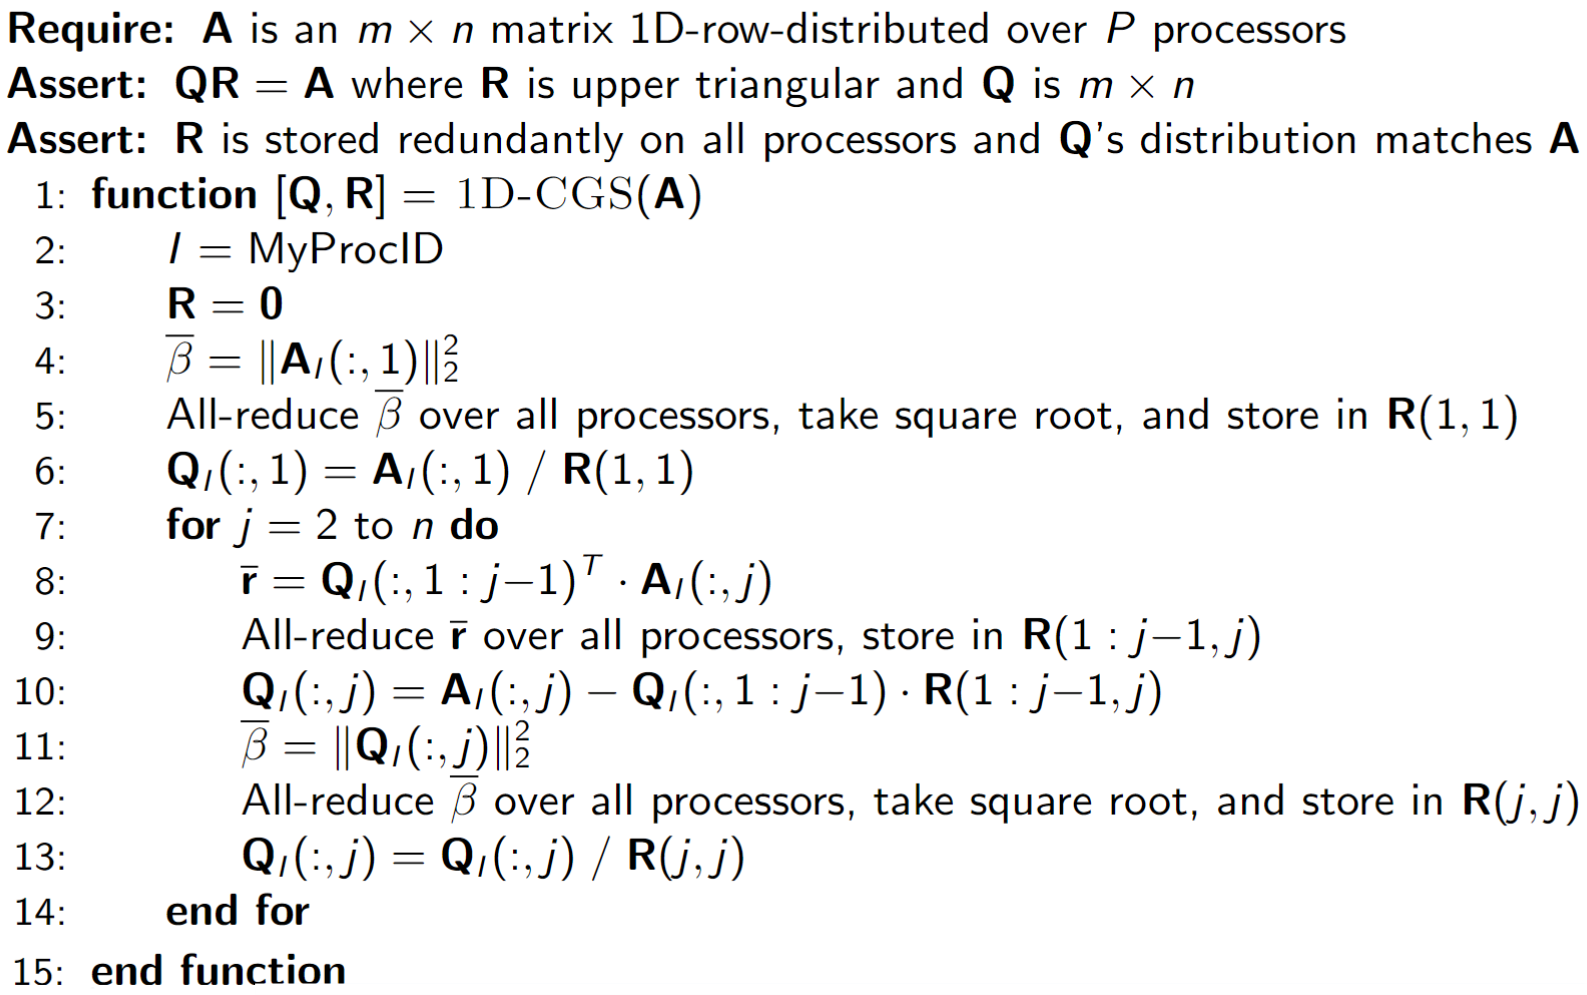
\includegraphics[width=.75\textwidth]{CGS_pseudocode}
					\caption{Pseudocode of parallelised CGS algorithm.}
					\label{fig:CGS-pseudocode}
			\end{figure}
		\subsection{Cholesky-QR}
			The pseudocode for parallel Cholesky-QR is given in \ref{fig:Cholesky-QR-pseudocode}.
			Parallel Cholesky-QR computes on every processor the $n\times n$ component $A_i^TA_i$ of $A^TA$. This is done by computing the local $A_i^TA_i$ and then summing the results with an Allreduce operation. The Cholesky decomposition is then computed on every processor as it is on a $n\times n$ matrix, and we want to limit unnecessary communication. The contribution $Q_i$ of processor $i$ to the $Q$ matrix is then computed by solving the system $R^TQ_i^T=A_i^T$. The final result is obtained by a Gather operation. 
			\begin{figure}
				\centering
				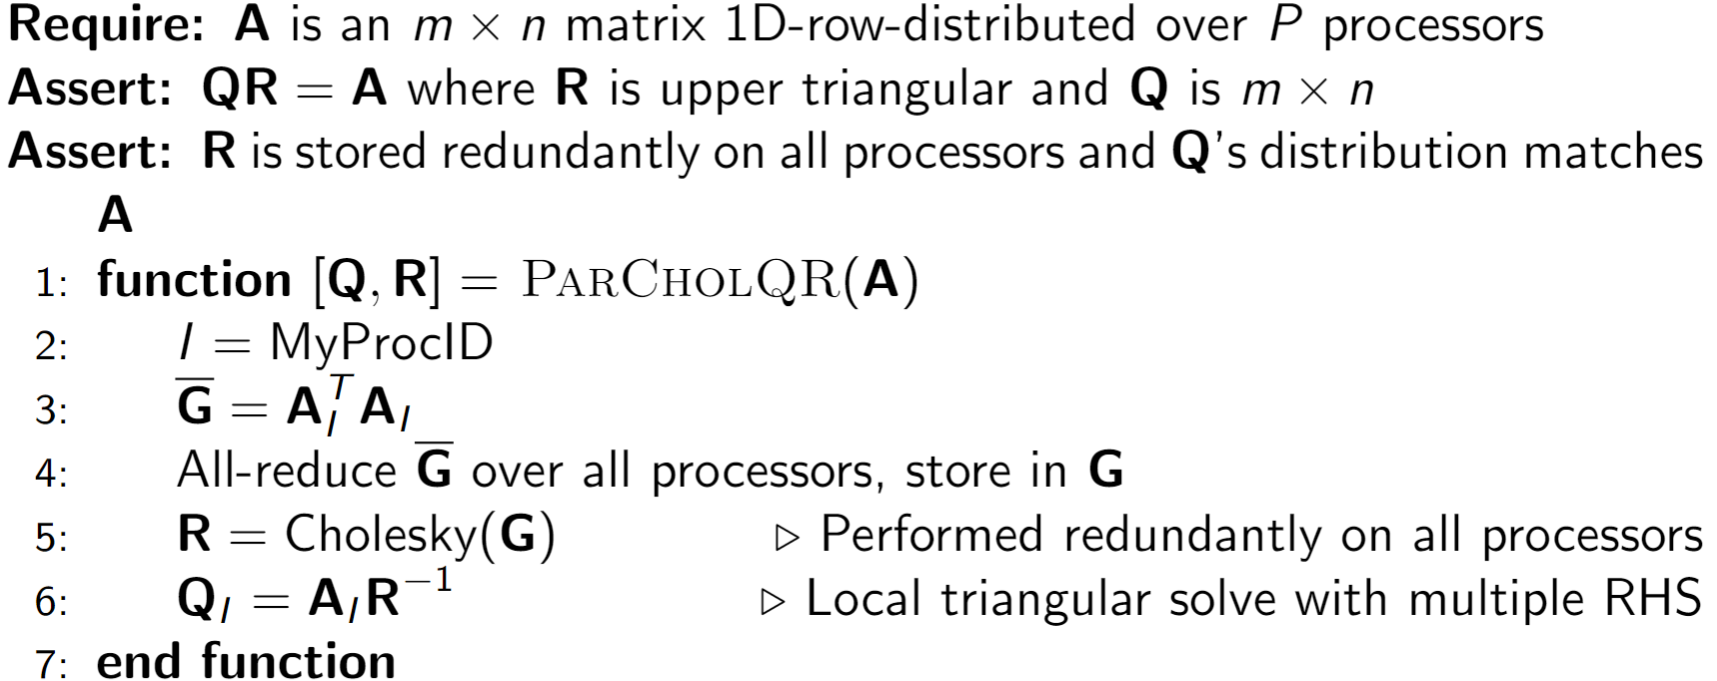
\includegraphics[width=.7\textwidth]{cholesky_QR_pseudocode}
				\caption{Pseudocode of parallelised Cholesky-QR algorithm.}
				\label{fig:Cholesky-QR-pseudocode}
			\end{figure}
		\subsection{TSQR}
			The pseudocode for TSQR is given in \ref{fig:TSQR-pseudocode}.
			TSQR was mostly explained already in the previous section. We might add that the reconstruction of the $Q$ matrix is done a posteriori by building the $Q^{(k)}$ matrices going up the binary tree and multiplying it by the trailing $Q^{(k-1)\leftarrow(0)}$ matrix. 
			\begin{figure}
				\centering
				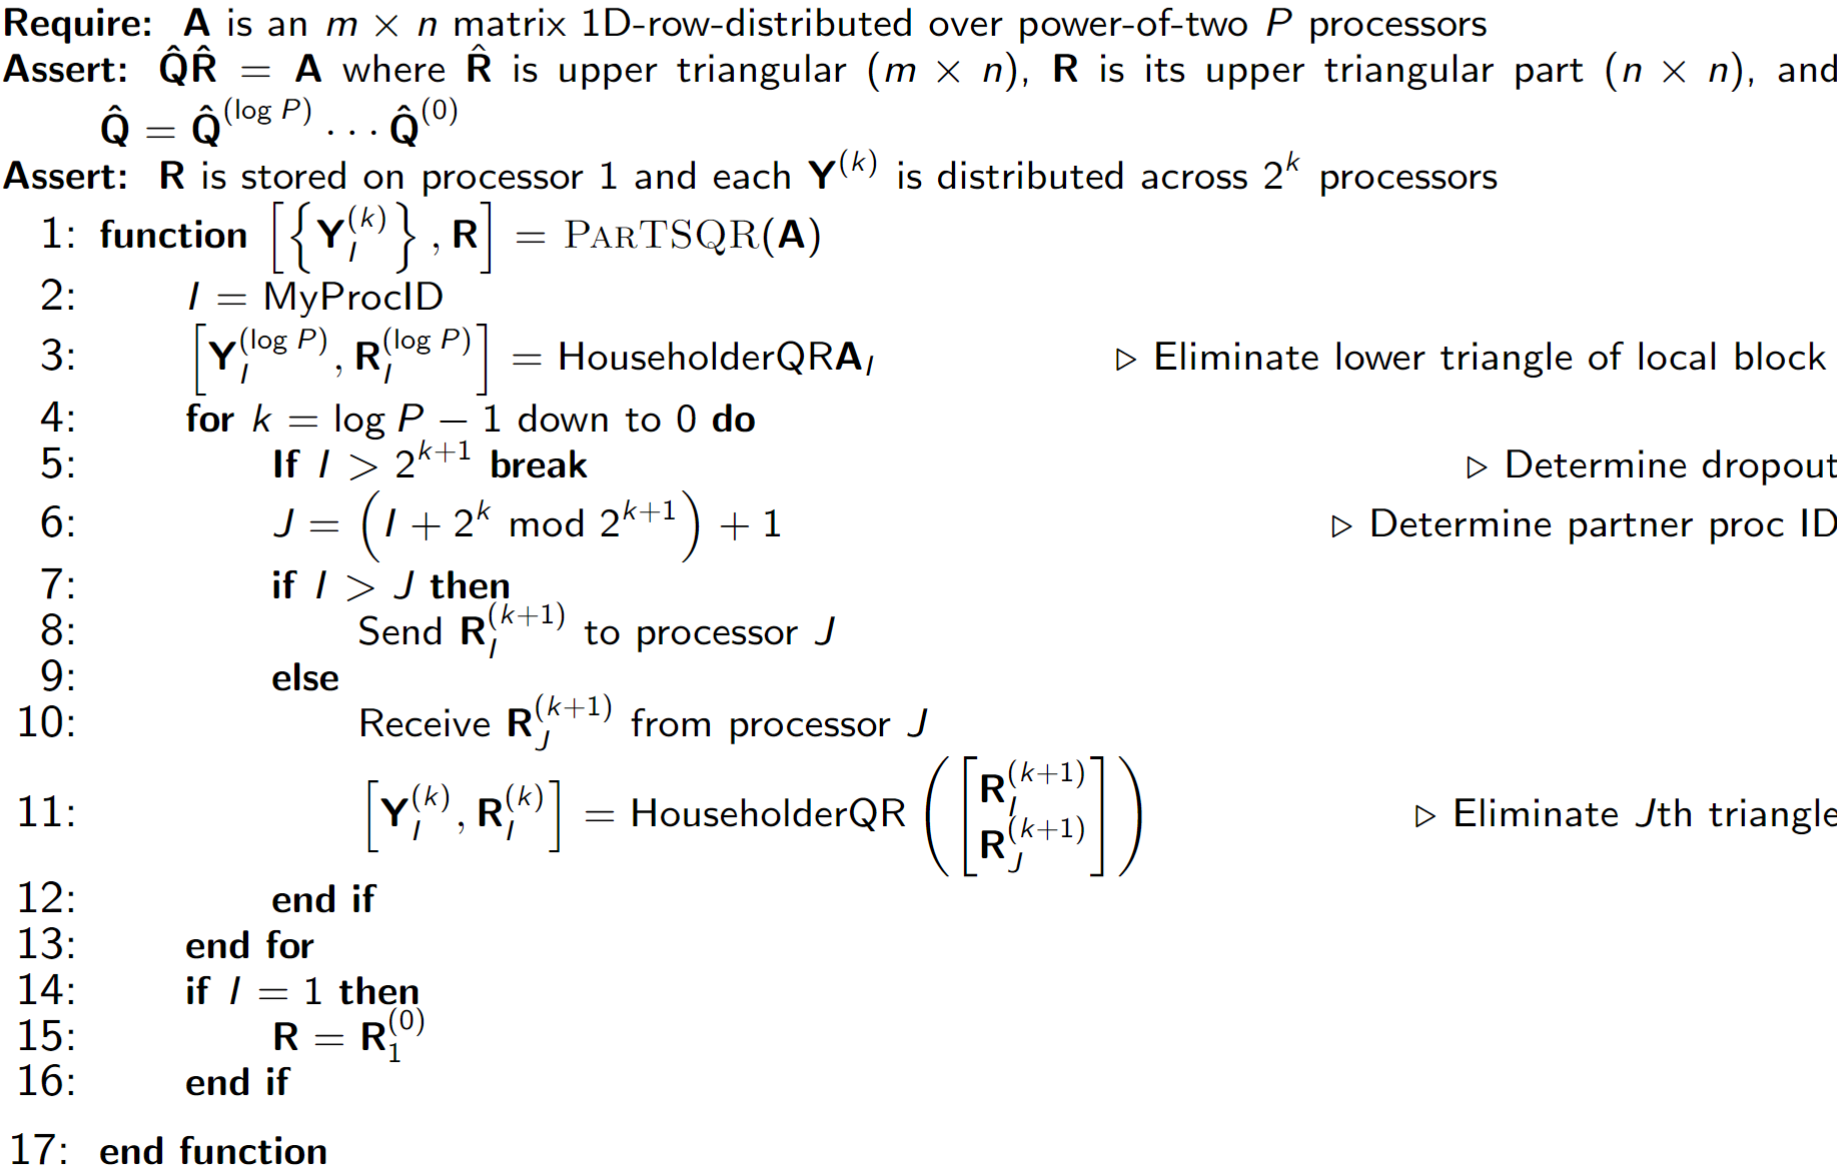
\includegraphics[width=.8\textwidth]{TSQR_pseudocode}
				\caption{Pseudocode of parallelised TSQR algorithm.}
				\label{fig:TSQR-pseudocode}
			\end{figure}
	
	\section{Experimental procedure}
		For all the presented results, we used $m=2^{15}=32768$ and $n=330$, unless stated otherwise. This choice was based on the fact that we wanted the computations of the metrics to take a reasonable time, while providing the algorithms with a sufficiently large matrix for the run times not to have too high of a variance.	

		For a theoretical investigation, the bounds on the loss of orthogonality provided in the lectures should be used. 
		\subsection{Chosen Matrices}
			The singular matrix, which we denote $C \in \mathbb{R}^{m \times n}$ was was generated by uniformly discretizing the following parametric function
			$$
			f(x, y)=\frac{\sin (10(y+x))}{\cos (100(y-x))+1.1}
			$$
			over the $0 \leq x, y \leq 1$ domain.

			The non singular matrix was obtained from the SuiteSparse Matrix Collection, https: //sparse.tamu.edu/about. More precisely, the ..., $k\times l$ ???  matrix was used. To make it $m\times n$, its first $m$ lines and $n$ columns were kept. 
		\subsection{Numerical Stability}
			For the numerical investigation, the loss of orthogonality is measured as $\left\|I-Q^T Q\right\|_2$ and the condition number of the basis $Q$. Indeed, the condition number of the basis $Q$ is also a measure of orthogonality since it is defined as the ratio of the largest and smallest singular values $\sigma_{\max{}},\sigma_{\min}$ of $Q$ and orthogonal matrices should have $|\sigma_i|=1\ \forall i$. 
		
			In general, these quantities where considered at the end of the algorithm. For CGS, however, as it is possible, an analysis of these quantities' evolution over the iterations of the algorithm when was also led.

			As Cholesky QR could not be run on big $C$ matrices due to numerical stability issues, we studied its behaviour as a function of matrix size for smaller sizes. This was done by considering the $C_s=C(m=2000s,5s)$ matrix for values of $s$ between 1 and 30, which made the condition number of $C_s$ vary from $10^1$ to $10^7$.
		\subsection{Runtimes}
			The run times where obtained by timing each processor $i$, and then taking the $\max{}$ over the processors. To quantify uncertainty and get a more accurate estimate, the run times were measured by repeating the computations $n_{\text{rep}}=5$ times.
			During the run time measurements, the number of processors was taken as powers of 2 between 1 and 64.
				
		Your report should state the theoretical bounds for the loss of orthogonality of the three algorithms. You should explain why these measures are important. For each matrix you should plot or put in a table the loss of orthogonality/condition number. You should explain these plots, reference them, and make connection with the theory.
	\section{Numerical Stability Investigation}
		\subsection{As a function of $n$}
		\begin{wrapfigure}[32]{r}{0.525\textwidth}
			\vspace{-1em}
			\centering
			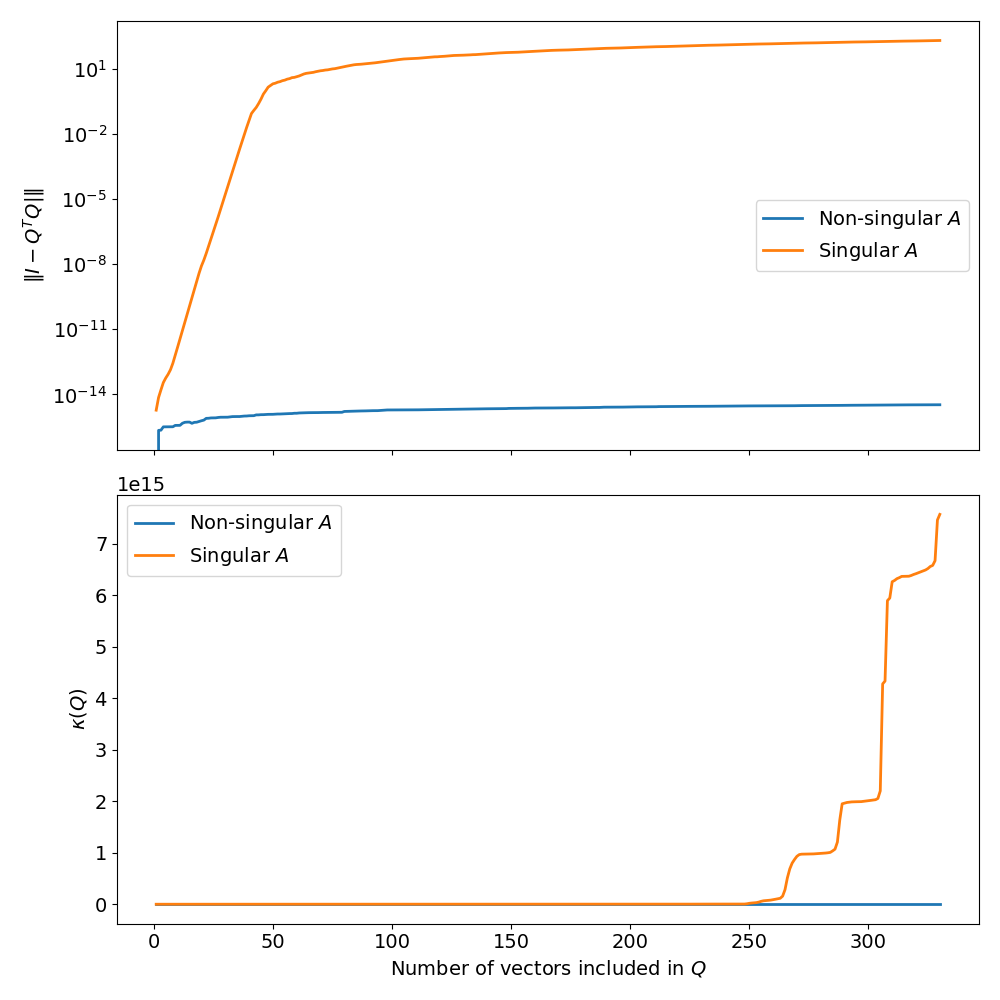
\includegraphics[width=.5\textwidth]{CGS_metric_evolution}
			\caption{Pseudocode of parallelised TSQR algorithm.}
			\label{fig:CGS-metric-evolution}
		\end{wrapfigure}
		The first thing we explore is the behaviour of the loss of orthogonality and condition number of the $Q$ matrix as a function of the number $n$ of vectors that are on the orthogonal basis. To do this, the metrics are computed for $n$ between 1 and 330, and the results are plotted on semi-log plots in \ref{fig:CGS-metric-evolution}.

		Looking at these plots, we see that both metrics explode for the singular matrix as a function on $n$. The loss of orthogonality actually behaves exponentially for small values of $n$ (i.e. up to $\sim 50$ or so), before plateauing at around 10. Both these behaviours can be understood as follows. (1.) The $n$th added vector needs to be orthogonal to $n-1$ other ones, and so contributes to $n-1$ numerical errors. (2.) The vectors are normed to $1$ and so the loss of orthogonality plateaus to a value characteristic of a random matrix under the same constraint. 

		The condition number has a more surprising curve. Indeed, there seem to be some really small plateaus whose structure repeats periodically with period $\sim 40$. I was not able to come up with a good explanation for this behaviour. Another interesting point to notice is that the condition number starts to increase only once the loss of orthogonality has exploded. This was, at least partly expected, as singular values of an orthogonal matrix are 1. 
		%\lipsum[1-4]
		\subsection{Algorithm comparison}
		We now compare the three algorithms between them. We do so by considering the loss of orthogonality and $Q$'s condition number at the end of the computation. The results are presented in \ref{tab:numberical-stability}.

		As a quick look to the table confirms, the observed behaviours are the expected ones. For the well conditioned matrix, all algorithms perform well, yielding a perfect condition number, and a loss of orthogonality of the order of machine precision. For the ill-conditioned matrix : TSQR perform just as well, as it is unconditionally stable; CGS fails, as the $Q$ matrix has a condition number of order $10^{15}$, and saturates the loss of orthogonality; while Cholesky QR runs into a fatal error, as it perceives the matrix as a singular one.
		
		From this analysis, we can conclude that TSQR is the only algorithm one should use if the matrix is ill-conditioned. For well-conditioned matrices, all algorithms are accurate.  
		\begin{table}[h]
			\centering
			\begin{tabular}{|c|l|c|c|c|}
			\hline
			Metric                            & Matrix Type & Cholesky QR & Classical Gram-Schmidt & Tall-skinny     \\ \hline
			\multirow{2}{*}{$\|I-Q^TQ\|$} & $\kappa(A)=1.984\times 10^{4}$  & 4.153$\times 10^{-15}$ & 3.350$\times 10^{-15}$ & 5.550$\times 10^{-15}$ \\ \cline{2-5} 
											  & $\kappa(A)=3.883\times 10^{15}$ & Error & 1.991$\times 10^{2}$ & 8.255$\times 10^{-15}$ \\ \hline
			\multirow{2}{*}{$\kappa(Q)$} & $\kappa(A)=1.984\times 10^{4}$  & 1 & 1 & 1 \\ \cline{2-5} 
											  & $\kappa(A)=3.883\times 10^{15}$ & Error & 7.572$\times 10^{15}$ & 1 \\ \hline
			\end{tabular}
			\caption{Metrics for numerical stability of the considered algorithms. The entry for the ill-conditioned matrix and Cholesky QR is marked as ``Error'' as the algorithm could not be run. Indeed, in this case the matrix was perceived as singular.}
			\label{tab:numberical-stability}
			\end{table}
			\subsection{Cholesky QR's stability : a deep dive}
			\begin{wrapfigure}[18]{r}{0.5\textwidth}
				\centering
				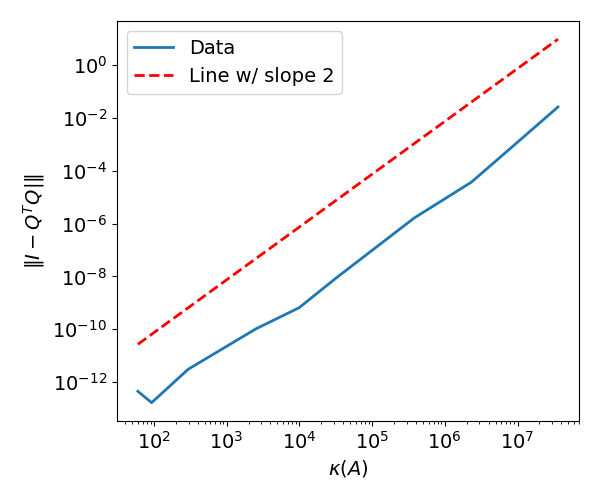
\includegraphics[width=.5\textwidth]{CQR_stability}
				\caption{Loss of orthogonality of the $Q$ matrix obtained by Cholesky QR as a function of input-matrix condition number.}
				\label{fig:CQR-stability}
			\end{wrapfigure}
			To better understand the numerical stability issues that Cholesky QR runs into, we now turn to its behaviour as a function of $A$'s condition number. The associated results are presented in a log-log plot in \ref{fig:CQR-stability}.
			Looking at the plot, we can see that the loss of orthogonality grows quadratically as a function of the condition number (the slope on a log-log plot is an exponent on a lin-lin plot). This observation is compatible with the theoretical prediction, as Cholesky QR makes use of the Cholesky decomposition of $A^TA$, which has condition number $\kappa(A^TA)=\kappa(A)^2$. This allows us to conclude that the algorithm will interpret matrices with a condition number above $10^8$ as if they where singular. ???
			%To better understand the Your report should state the theoretical bounds for the loss of orthogonality of the three algorithms. You should explain why these measures are important. For each matrix you should plot or put in a table the loss of orthogonality/condition number. You should explain these plots, reference them, and make connection with the theory.
	\section{Runtime Investigation}
		\begin{wrapfigure}[32]{r}{0.5\textwidth}
			\centering
			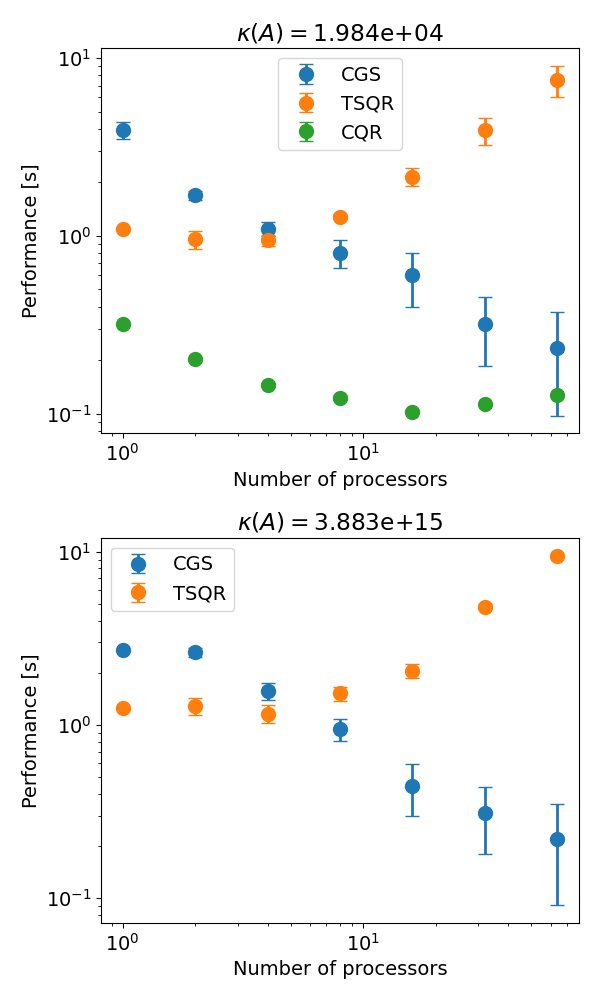
\includegraphics[width=.5\textwidth]{runtime_vs_nprocs}
			\caption{Pseudocode of parallelised TSQR algorithm.}
			\label{fig:runtime-vs-nprocs-mat}
		\end{wrapfigure}	
		\lipsum[1-2]

	\section{Conclusion}
	\section*{Aknowledgements}
	
	\appendix
		\section{Runtime Estimation}\label{appendix:runtime_estimation}
		%\input{elasticity_discussion.tex}	
	%\begin{wrapfigure}[30]       % replace <line_nb> the with number of lines for the wrapping
	%	\centering                                          % and <side> by r or l for right or left (position on the page)
	%		\vspace{0em}
	%		\includegraphics[width=\textwidth]{yields_vs_T_for_diff_t}
	%		\caption{This is a caption}
	%		\label{fig:yield_vs_T_for_diff_t}
	%\end{wrapfigure}
	%\medskip
	%\titleformat*{\section}{\normalfont\large\bfseries}
	%\printbibliography[heading=bibintoc,title={Bibliography}] 
%	\vspace*{\fill}
%%%
\end{document} 